\documentclass[11pt, a4paper, pdf]{article}
\newcounter{minitocdepth}
\newcounter{chapter}
\newcommand{\chaptername}{}

%\include{estil-llibre}
\usepackage{iesbbook}

\renewcommand{\hot}[1][]{
	\ifthenelse{\equal{#1}{}}{$\mathbf{\bigstar}$ \underline{\textbf{LLIBRE}}: }{\myrepeat{#1}{$\mathbf{\bigstar}$}}
}
 \renewcommand{\normalsize}{\fontsize{10.5}{11.2}\selectfont}
 
 \fancypagestyle{blocfancy}{
 	\pagestyle{fancy}% Duplicate fancy page style
 	\fancyhead{} % clear all header fields
 	\fancyhead[RE,LO]{{IES Binissalem. Matemàtiques 2n BATX}}
 	\fancyhead[LE,RO]{\bfseries\large\thepage}
 }
\let\ofrac\frac
\let\frac\dfrac
\begin{document}
\pagestyle{blocfancy}
\setcounter{myenumi}{0}
\begin{center}
	\large
	\textbf{\underline{
	Feina d'estiu per als alumnes que han de cursar Matemàtiques II al batxillerat.
	}
	}
\end{center}



\begin{blueshaded}
		\textbf{Instruccions: } Realitzau en un quadern (pot ser el mateix que fareu servir per l'assignatura durant el proper curs) les activitats proposades en aquest dossier. Aquesta feina es presentarà al professor del proper curs durant els primers dies de classe. La realització correcta d'aquesta tasca serà valorada com una nota de la primera avaluació.
		
		\textbf{Ajuda: } Si necessitau ajuda podeu consultar els apunts o el llibre de text Matemàtiques I i els recursos penjats a https://piworld.es. 
\end{blueshaded}

\section{Sistemes lineals}

\begin{mylist}
 

	\item Resoleu aquests sistemes pel mètode de Gauss
 \begin{tasks}(2)
	\task  $\left\{\begin{array}{ll} x+y+z&=2 \\ x-y+z&=6 \\ x-y-z&=0 \end{array}\right. $       
	\task  $\left\{\begin{array}{ll} 2x+3y&=14 \\ x-2y+z&=-3 \\ 2x-y-z&=9 \end{array}\right. $ 
	\task  $\left\{\begin{array}{ll} 5x-4y+3z&=9 \\ 2x+y-2z&=1 \\ 4x+3y+4z&=1 \end{array}\right. $        
	\task  $\left\{\begin{array}{lll} 2x-5y&+4z&=-1 \\ 4x-5y&+4z&=3 \\ 5x&-3z&=13 \end{array}\right. $ 
\end{tasks}
	
	
	\item Classifiqueu en (S.C.D, S.C.I, S.I) i resoleu, quan sigui possible, aquests sistemes pel mètode de Gauss
	\begin{tasks}(2)
		\task  $\left\{\begin{array}{ll} x-y&=1 \\ 2x+6y-5z&=-4 \\ x+y-z&=0 \end{array}\right. $       
		\task  $\left\{\begin{array}{ll} x+2y+z&=3 \\ x-2y+5z&=5 \\ 5x+22y+17z&=1 \end{array}\right. $ 
		\task  $\left\{\begin{array}{ll} x+y+3z&=2 \\ 2x+3y+4z&=1 \\ -2x-y-8z&=-7 \end{array}\right. $        
		\task  $\left\{\begin{array}{ll} 2x-y-z&=2 \\ 3x-2y-2z&=2 \\ -5x+3y+5z&=-1 \end{array}\right. $ 
		\task  $\left\{\begin{array}{ll} x+y+z&=3 \\ -x+2y+z&=5 \\ x+4y+3z&=1 \end{array}\right. $ 
		\task  $\left\{\begin{array}{ll} -2x+y+z&=1 \\ 3x+2y-z&=0 \\ -x+4y+z&=2 \end{array}\right. $ 
	\end{tasks}
	 
	
	\item Una prova tipus test consta de 30 preguntes. Cada pregunta ben contestada suma 5 punts, cadascuna mal contestada resta 2 punts i les deixades en blanc no penalitzen. Si l'alumne hagués deixat en blanc 3 preguntes mal contestades, tindria igual nombre de cada tipus. Si sabem que l'alumne va obtenir 72 punts a la prova, quantes preguntes be, malament i en blanc va contestar? 
	
	\item Tres germans, na Maria, en Joan i en Pere, decideixen regalar un ram de flors de 18.75 euros a la seva mare pel seu aniversari. Reuneixen aquesta quantitat de forma que na Maria aporta la meitat del que aporten els altres dos plegats i en Joan aporta 3 euros per cada 2 que n’aporta en Pere. Quina quantitat aporta cada un dels germans? 
	
	\item Es tenen 1385 \euro en bitllets de 5, 20 i 100 \euro. El nombre de bitllets de 5 \euro excedeix en 7 unitats el nombre de bitllets de 100 \euro. Per cada 2 bitllets de 100 \euro se’n tenen 3 de 20 \euro. Quants de bitllets hi ha de cada valor? 
	
			
\end{mylist}	 
	 
	 
\section{Derivades}

\begin{mylist}
	
	\item Calculeu i simplifiqueu les \underline{derivades primeres} de les següents funcions
	\begin{tasks}(2)
		\task  $y=\frac{x}{x^2-4} + \frac{\ln (x+1)}{x+1}$
		\task $y=x\cdot e^{x^2}$
		\task $y = \frac{\sqrt[3]{x^2}}{ x \sqrt{x} }$
		\task $y = x \cdot \sqrt{4+5x^2}$
		\task  $y=\frac{1}{2}\tg^2 (5x^2+\ln x)$
		\task  $y=x^3 \cdot (\arctg x - x) $
	\end{tasks}
	
	\item Calculeu i simplifiqueu les \underline{derivades segones} de les següents funcions
	\begin{tasks}(2)
		\task $y=\cos (3 x^2+2x-1)$
		\task $y=\frac{\sin x}{x}$
		\task $y=x\cdot (e^{-x}+1)$
		\task $y=\frac{2x+1}{(x^2+x+1)^2}$
	\end{tasks}
\end{mylist}


\section{Representació de funcions}

\begin{mylist}
	
	\item Feis un estudi complet de les funcions següents (domini, punts de tall, asímptotes, màxims, mínims, etc.)
 i representeu-les gràficament
 \begin{tasks}(3)
 	\task $y=x^3-3x^2+2$
 	\task $y=-x^4+2x^2+3$
 	\task $y=\frac{1+x}{1-x}$
 	\task $y=\frac{x^2-1}{x^2-4}$
 	\task $y=\frac{x^4+1}{x^3}$
 	\task $y=x^2 \cdot e^x $
 \end{tasks}
 
 
 	\item Calculau el punt sobre la recta $2x+y=3$ tal que el producte de les seves coordenades sigui màxim.
 	
 	\item Calculeu l'equació de la recta tangent a $y=5x^2+3x-2$ en $x=-1$.
 	
 	\item Calculeu l'equació de la recta tangent a la corba $y=x^3-6x^2+1$ en el seu punt d'inflexió.
 	
 	\item Trobau els extrems relatius de la funció $f(x)=\frac{1}{x+1} +\frac{x}{x+4}$.
 		
\end{mylist}

\section{Probabilitat elemental}

\begin{theorybox}
	Es tracta que repasseu la probabilitat elemental d'ESO. Entreu a https://piworld.es i visualitzeu els vídeos núm. 155, 156, 157 i 158 sobre probabilitat elemental.	
\end{theorybox}

\begin{mylist}
 
 \item Utilizant la regla de Laplace, calcula aquestes probabilitats elementals
 \begin{tasks}
 	\task Treure múltiple de 3 en llançar un dau cúbic.
 	\task Treure més de 7 en llançar un dau dodecaèdric (12 cares iguals).
 	\task Treure rei de bastos d'una baralla espanyola de 40 cartes.
 	\task Treure un bolígraf vermell d'un estoig que conté 10 bolis negres, 3 de blaus i 2 vermells.
 	\task Endevinar la xifra de les desenes d'un nombre de 3 xifres.
	\task Que la suma de les dues darreres xifes del nombre sigui 11.
 	\task Treure una fitxa doble en un joc de dominó de 28 fitxes.
 \end{tasks}

\item Es tria a l'atzar un nombre natural a partir de l'1 fins el 50. Definim els successos:

\quad $A$=``Sortir un número major que 4 i menor que 17''.

\quad $B$=``Sortir un quadrat perfecte''

Calcula les probabilitats $P(A)$, $P(B)$, $P(A\cap B)$ i $P(A\cup B)$. \textit{Nota:  La intersecció $A\cap B$ significa que passin els dos successos simultàniament. La unió $A\cup B$ significa que passin almenys un dels dos successos.}

\item 
Joan, Lluís, Aina i Pere jugaran al parxís. Per veure qui comença el joc, cadascun
d'ells tira un dau. Si Joan ha tret un 5, Lluís un 3 i Aina un 4, troba la probabilitat que en Pere obtingui un resultat:
\begin{tasks}(3)
\task Diferent al dels altres. \task Superior a tots. \task Inferior a tots.
\end{tasks}

\item Llançam un moneda 3 vegades. Calcula la probabilitat:
	a) Treure 3 cares.
	b) Treure 2 cares.
 \textit{Ajuda: Dibuixa un diagrama d'arbre.}

\item Tenim una urna que conté 3 bolles blanques i 7 bolles negres. Treim dues bolles amb reemplaçament, calcula la probabilitat:
\begin{tasks}(2)
	\task d'obtenir almenys 1 bolla blanca
	\task d'obtenir bolles d'igual color
\end{tasks}
Repetiu per sense reemplaçament. \textit{Ajuda: Dibuixa un diagrama d'arbre.}


\item  Posam les lletres de la paraula LLAPIS en una bossa i en treim dues sense reemplaçament. a) Quina és la probabilitat de treure dues vocals? b) I una vocal i una consonant? 

\item 
Davant d'un examen, un alumne només ha estudiat 15 dels 25 temes. Aquest es realitza extraient a l'atzar dos temes i deixant que l'alumne esculli un dels dos. Trobau la probabilitat que l'alumne hagi estudiat almenys un dels dos temes.
\end{mylist}
 
\section*{Solucions}
\setcounter{myenumi}{0}
\begin{multicols}{2}
\begin{mylist}
 
 \item  \begin{tasks}
 	\task $x=1$; $y=-2$; $z=3$ 
 	\task $x=4$; $y=2$; $z=-3$ 
 	\task $x=1$; $y=-1$; $z=0$ 
 	\task $x=2$; $y=1/5$; $z=-1$ 
 \end{tasks}
 
 \item 
 \begin{tasks}
 	\task S.C.D. $x=3/2$; $y=1/2$; $z=2$ 
 	\task S.I. no té solució. 
 	\task S.C.I. $x=5-5z$; $y=2z-3$; $z=z$ 
 	\task S.C.D. $x=2$; $y=1/2$; $z=3/2$
 	\task S.I. no té solució.
 	\task S.C.I. $x=1-3y$; $y=y$; $z=3-7y$
 \end{tasks}
  
 \item Be 18, Malament 9, en blanc 3
 
 \item Maria 6,35 \euro, Joan 7,5 \euro, Pere 5 \euro
 
 \item Planteig: $5x+20y+100z=1385$, $x=7+z$, $\frac{z}{2}=\frac{y}{3}$. Solució: $x=17$, $y=15$, $z=10$.
 
 \item \begin{tasks}
 	\task  $y'=\frac{-1}{x^2-4} + \frac{1-\ln(x+1)}{(x+1)^2}$ 
 	\task $y'=(1+2x^2)\cdot e^{x^2}$
 	\task $y'=-\frac{5}{6\sqrt[6]{x^{11}}}$
 	\task $y'=\frac{4+10x^2}{\sqrt{4+5x^2}}$
 	\task $y'=\frac{\tg(5x^2+\ln x) }{\cos^2(5x^2+\ln x)}\cdot (10x+\frac{1}{x})$
 	\task $y'=3x^2(\arctg x - x) - \frac{x^5}{1+x^2}$
 \end{tasks}

\item \begin{tasks}
	\task $y'=-(6x+2) \cdot \sin(3x^2+2x-1)$
	
	$y''=-6\,\sin(3x^2+2x-1)- (6x+2)^2\, \cos(3x^2+2x-1)$
	%
	\task $y'=\frac{x\cdot \cos x + \sin x}{x^2}$
	
	$y''=\frac{-(x^2+2)\, \sin x}{x^3}$
	%
	\task $y'=(1-x)\, e^{-x} + 1$
	
	$y''=(x-2) \, e^{-x}$
	%
	\task $y'=\frac{-6(x^2+x)}{(x^2+x+1)^3}$
	
	$y''=\frac{24x^3+36x^2-6}{(x^2+x+1)^4}$
\end{tasks}

\item  
	\begin{center} a)
	 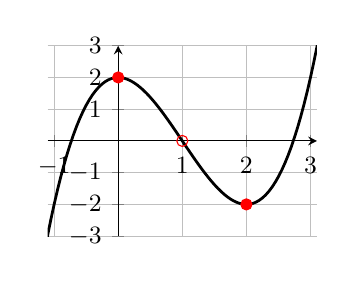
\begin{tikzpicture}[]
	\begin{axis}[width=5cm,height=4cm, axis background/.style={fill=white}, axis lines=middle, 
	grid = major,
	xtick={-5,-4,...,3},
	ytick={-3,-2,...,3},
	ymin = -3,
	ymax = 3,
	tick label style={font=\small},
	legend style={font=\small,legend pos=outer north east},]
	\addplot[ samples=201, line width=1pt]{x^3-3*x^2+2}; 
	\addplot[red, mark=*, only marks] coordinates{(0,2) (2,-2)};	
	\addplot[red, mark=o, only marks] coordinates{(1,0)};
	\end{axis}
	\end{tikzpicture}
	\end{center}
%%
\begin{center} b)
	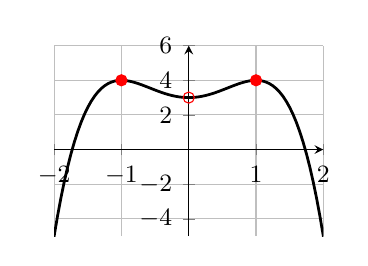
\begin{tikzpicture}[]
	\begin{axis}[width=5cm,height=4cm, axis background/.style={fill=white}, axis lines=middle, 
	grid = major,
	xtick={-5,-4,...,3},
	ytick={-4,-2,...,6},
	ymin = -5,
	ymax = 6,
	tick label style={font=\small},
	legend style={font=\small,legend pos=outer north east},]
	\addplot[ samples=201, line width=1pt]{-x^4+2*x^2+3}; 
	\addplot[red, mark=*, only marks] coordinates{(-1,4) (1, 4)};	
	\addplot[red, mark=o, only marks] coordinates{(0,3)};
	\end{axis}
	\end{tikzpicture}
\end{center}
%% 
\begin{center}c)
	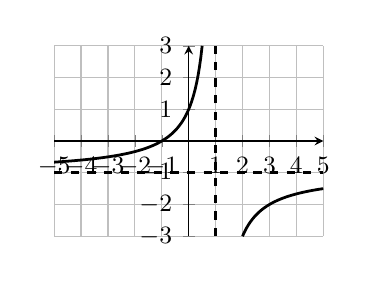
\begin{tikzpicture}[]
	\begin{axis}[width=5cm,height=4cm, axis background/.style={fill=white}, axis lines=middle, 
	grid = major,
	xtick={-5,-4,...,5},
	ytick={-3,-2,...,3},
	ymin = -3,
	ymax = 3,
	restrict y to domain=-3:3,
	tick label style={font=\small},
	legend style={font=\small,legend pos=outer north east},]
	\addplot[ samples=201, line width=1pt]{(1+x)/(1-x)}; 
	\addplot[no marks, dashed,  line width=1pt] coordinates{(-5,-1) (5, -1)};
 	\addplot[no marks, dashed,  line width=1pt] coordinates{(1,-3) (1, 3)};
	\end{axis}
	\end{tikzpicture}
\end{center}
%%
\begin{center}d)
	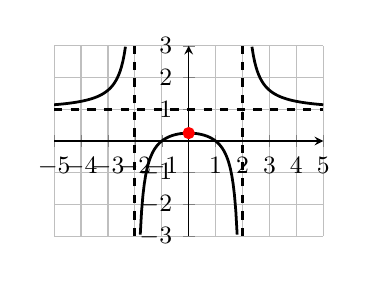
\begin{tikzpicture}[]
	\begin{axis}[width=5cm,height=4cm, axis background/.style={fill=white}, axis lines=middle, 
	grid = major,
	xtick={-5,-4,...,5},
	ytick={-3,-2,...,3},
	ymin = -3,
	ymax = 3,
	restrict y to domain=-3:3,
	tick label style={font=\small},
	legend style={font=\small,legend pos=outer north east},]
	\addplot[ samples=201, line width=1pt]{(x^2-1)/(x^2-4)}; 
	\addplot[red, mark=*, only marks] coordinates{(0,0.25)};	
	\addplot[no marks, dashed,  line width=1pt] coordinates{(-2,-3) (-2, 3)};
	\addplot[no marks, dashed,  line width=1pt] coordinates{(2,-3) (2, 3)};
	\addplot[no marks, dashed,  line width=1pt] coordinates{(-5,1) (5, 1)};
	\end{axis}
	\end{tikzpicture}
\end{center}
%%
\begin{center} e)
	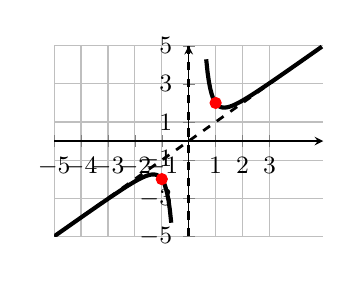
\begin{tikzpicture}[]
	\begin{axis}[width=5cm,height=4cm, axis background/.style={fill=white}, axis lines=middle, 
	grid = major,
	xtick={-5,-4,...,3},
	ytick={-5, -3,...,5},
	restrict y to domain=-5:5,
	tick label style={font=\small},
	legend style={font=\small,legend pos=outer north east},]
	\addplot[ samples=201, line width=1.5pt]{(x^4+1)/x^3}; 
	\addplot[red, mark=*, only marks] coordinates{(1,2) (-1,-2)};	
 	\addplot[no marks, dashed,  line width=1pt] coordinates{(-5,-5) (5, 5)};
\addplot[no marks, dashed,  line width=1pt] coordinates{(0,-5) (0, 5)};
	\end{axis}
	\end{tikzpicture}
\end{center}
%%
\begin{center} f)
	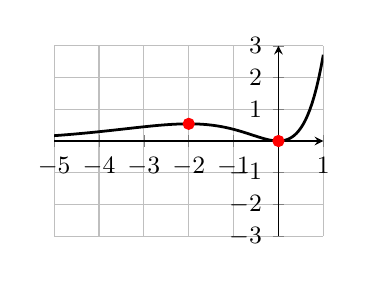
\begin{tikzpicture}[]
	\begin{axis}[width=5cm,height=4cm, axis background/.style={fill=white}, axis lines=middle, 
	grid = major,
	xtick={-5,-4,...,3},
	ytick={-3,-2,...,3},
	ymin = -3,
	ymax = 3,
	restrict y to domain=-3:3,
	tick label style={font=\small},
	legend style={font=\small,legend pos=outer north east},]
	\addplot[ samples=201, line width=1pt]{x^2*exp(x)}; 
	\addplot[red, mark=*, only marks] coordinates{(0,0) (-2,0.5413)};	
	\end{axis}
	\end{tikzpicture}
\end{center}

\item Cercau el màxim de $f(x)=x\cdot (3-2x)$ $x=3/4$, $y=3/2$

\item $y-0=-7(x+1)$

\item El punt d'inflexió és a $x=2, y=-15$. La recta tangent $y+15=-12(x-2)$

\item Derivada simplificada $y'=\frac{3x^2-12}{(x+1)^2 \,(x+4)^2)}$. Té un màxim a $x=-2, y=-2$ i un mínim a $x=2, y=2/3$

\item Correcció del professor.

\item $P(A)=6/25$; $P(B)=7/50$; $P(A\cap B)=1/25$; ; $P(A\cup B)=17/50$   

\item a) $P=\frac{3}{6}$, b) $P=\frac{1}{6}$,  c) $P=\frac{2}{6}$

\item Amb reemplaçament: a) $P=0,51$, b) $P=0,58$. Sense: a) $P=0,533$, b) $P=0,533$

\item a) $P=1/8$, b) $P=3/8$.

\item a) $P=2/30$, b) $P=16/30$.

\item $P=0.85$
\end{mylist}

\end{multicols}

\end{document}

